\chapter{Resultados}
\label{ch:resultados}

En el capitulo \ref{ch:metodos} presentamos la t\'ecnica de 
\textit{bootstraping}; el m\'etodo de Moreno-Dominguez para agrupar
tractogramas junto con algunas de sus falencias te\'oricas y como
solucionarlas usando la funci\'on \textit{logit}. En la secci\'on 
\ref{ch:nuestro}, presentamos nuestro m\'etodo para parcelar la corteza en
su totalidad. En las siguientes secciones mostramos primero los resultados
obtenidos al estudiar la estabilidad de los tractogramas; luego parcelamos
el \'area de Broca con ambos m\'etodos y finalmente parcelamos el
hemisferio derecho usando tambi\'en ambos m\'etodos. Todos los estudios se
realizaron sobre una misma mujer diestra de entre 23 y 26 a\~nos. Sus datos
fueron descargados de la base de datos \textit{Human Connectome Project}
\cite{VanEssen2012}. \\


\section{Estabilidad tractogramas}

Las Figuras \ref{fig:m1}, \ref{fig:m2} y \ref{fig:m3} muestran, para tres semillas
distintas, cinco cortes axiales del tractograma que se consigue al utilizar quince
mil part\'iculas.\\

Las Figuras \ref{fig:s1}, \ref{fig:s2} y \ref{fig:s3} muestran la varianza de 
cada voxel dentro de un mismo corte axial. La varianza se calcul\'o generando
mil tractogramas desde distinto n\'umero de streamlines. \\

La Figura \ref{fig:mv} muestra la media y varianza de los voxels $A$, $B$ y $C$
marcados en las Figuras \ref{fig:s1}, \ref{fig:s2} y \ref{fig:s3}. Estos voxels
fueron los que mayor varianza presentaron al generar tractogramas con dos mil
\textit{streamlines}.


\begin{figure}[h!]
   \centering
    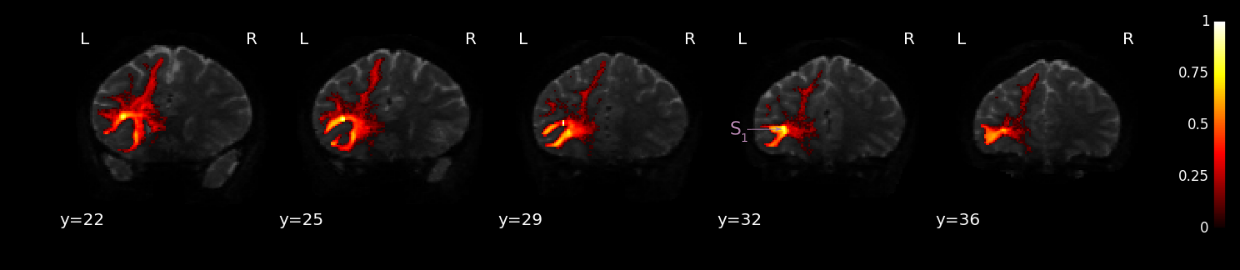
\includegraphics[width=\textwidth]{img/m1.png}
    \caption{Tractograma para la semilla $S1$ utilizando toda la muestra.}
    \label{fig:m1}
\end{figure}

\begin{figure}[h!]
   \centering
    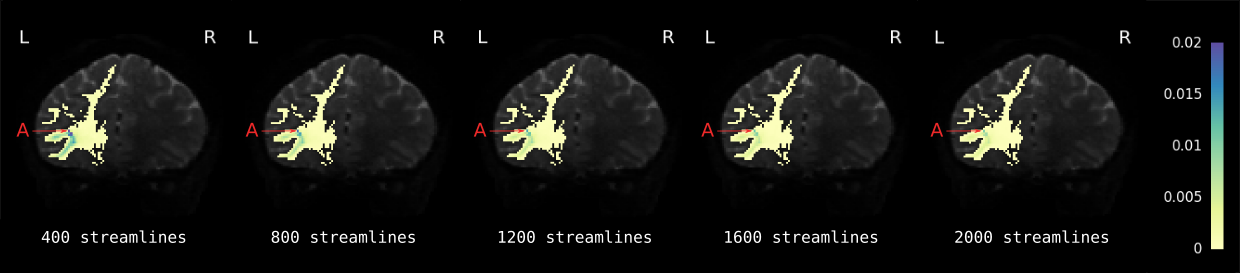
\includegraphics[width=\textwidth]{img/s1.png}
    \caption{Desviaci\'on Estandar respecto a la semilla $S1$. Mismo corte axial
             variando el tama\~no de las submuestras.}
    \label{fig:s1}
\end{figure}

\begin{figure}[h!]
   \centering
    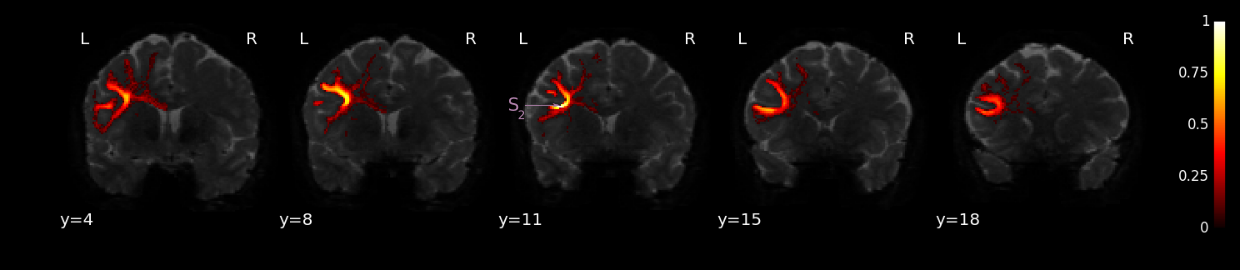
\includegraphics[width=\textwidth]{img/m2.png}
    \caption{Tractograma para la semilla $S2$ utilizando toda la muestra.}
    \label{fig:m2}
\end{figure}

\begin{figure}[h!]
   \centering
    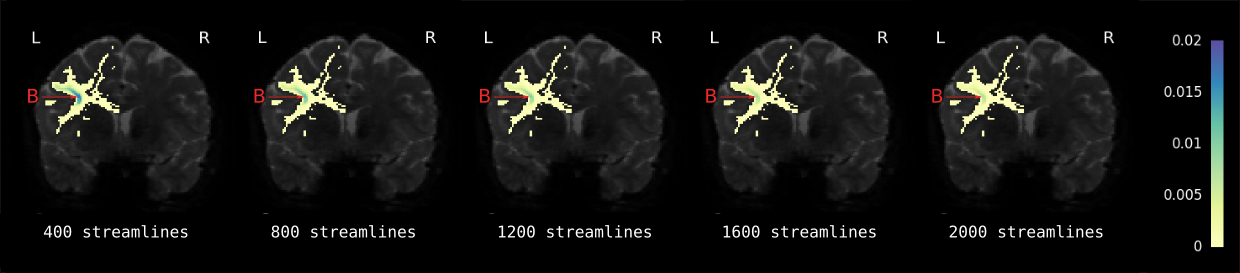
\includegraphics[width=\textwidth]{img/s2.png}
    \caption{Desviaci\'on Estandar respecto a la semilla $S2$. Mismo corte axial
             variando el tama\~no de las submuestras.}
    \label{fig:s2}
\end{figure}

\begin{figure}[h!]
   \centering
    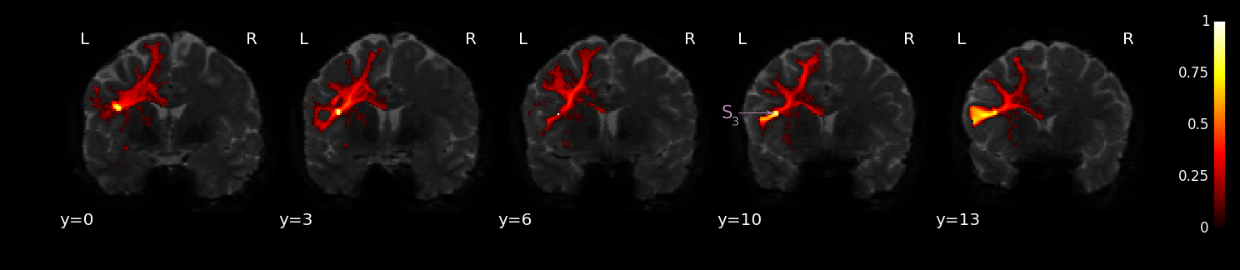
\includegraphics[width=\textwidth]{img/m3.png}
    \caption{Tractograma para la semilla $S3$ utilizando toda la muestra}
    \label{fig:m3}
\end{figure}

\begin{figure}[h!]
   \centering
    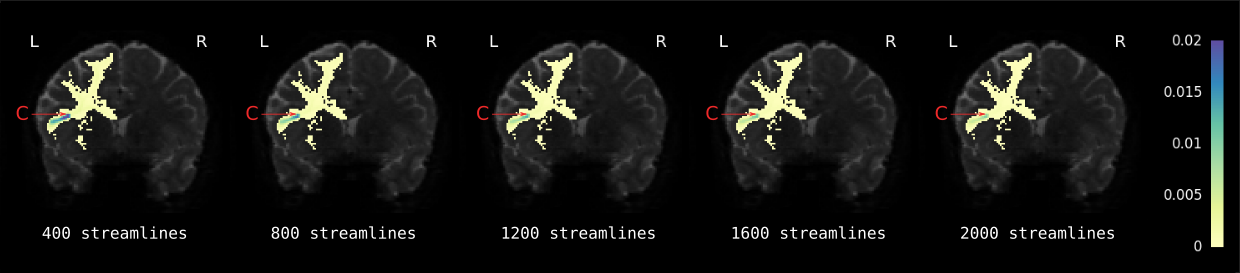
\includegraphics[width=\textwidth]{img/s3.png}
    \caption{Desviaci\'on Estandar respecto a la semilla $S3$. Mismo corte axial
             variando el tama\~no de las submuestras.}
    \label{fig:s3}
\end{figure}

\begin{figure}[h!]
   \centering
    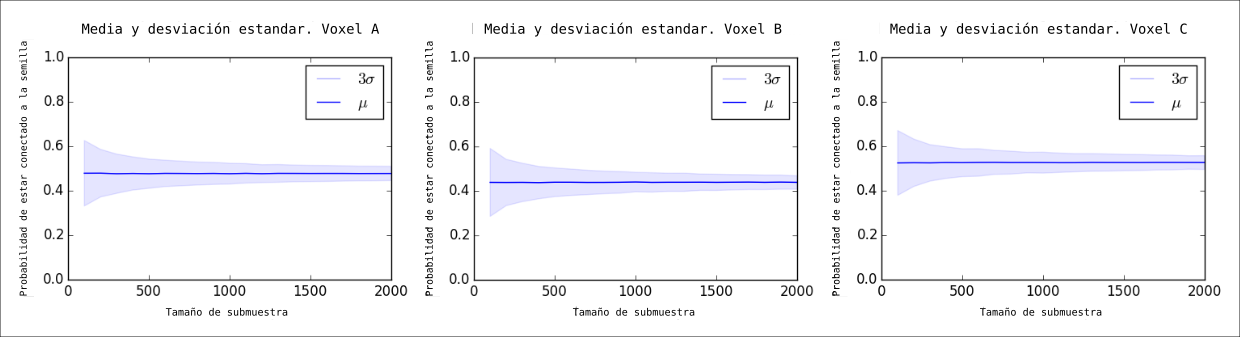
\includegraphics[width=\textwidth]{img/med_var_all.png}
    \caption{Media y desviaci\'on estandar de los voxels con mayor varianza.}
    \label{fig:mv}
\end{figure}


\section{Parcelando el \'Area de Broca}

\subsection{Distancia coseno con centroide}

Las siguientes Figuras muestran los resultados obtenidos al parcelar el \'Area
de Broca utilizando el m\'etodo de Moreno-Dominguez.

\begin{figure}[h!]
                                                                                                                        
\begin{minipage}[b]{\textwidth}
    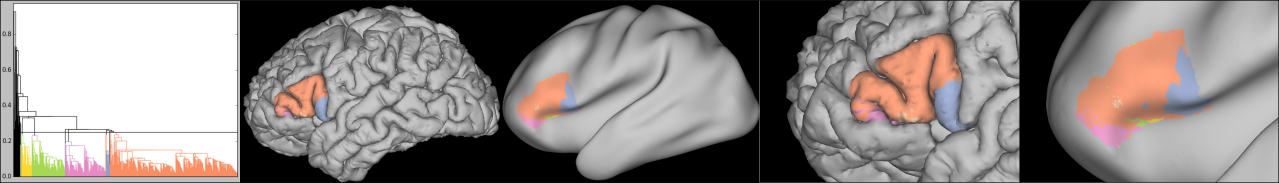
\includegraphics[width=\textwidth]{img/broca/moreno_0.png}
    \caption{M\'etodo Moreno sin preprocesamiento}

\end{minipage} ~
                                                                                                                       
\begin{minipage}[b]{\textwidth}
    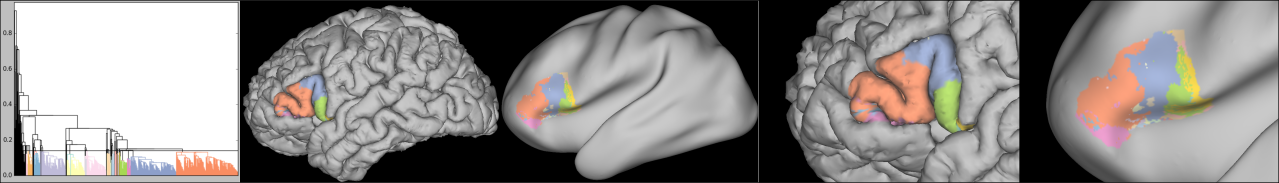
\includegraphics[width=\textwidth]{img/broca/moreno_0_deep.png}
    \caption{M\'etodo Moreno sin preprocesamiento, mayor profundidad en el 
            dendrograma}

\end{minipage} ~

\begin{minipage}[b]{\textwidth}
    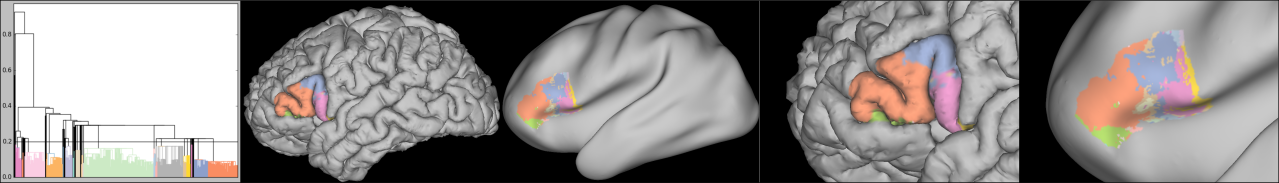
\includegraphics[width=\textwidth]{img/broca/moreno_400.png}
    \caption{M\'etodo Moreno, cuatrocientos pasos de preprocesamiento}

\end{minipage} ~

\begin{minipage}[b]{\textwidth}
    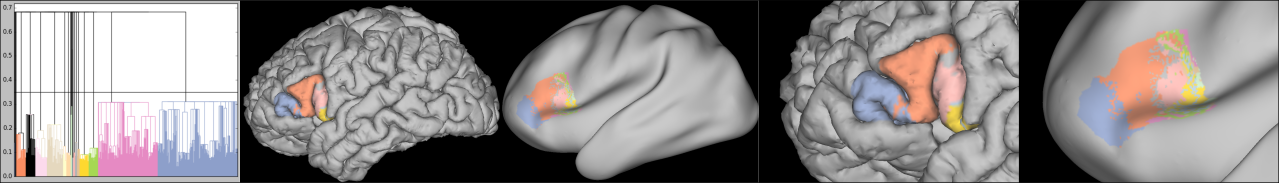
\includegraphics[width=\textwidth]{img/broca/moreno_750.png}
    \caption{M\'etodo Moreno, setecientos pasos de preprocesamiento}

\end{minipage} ~

\end{figure} 


\subsection{Utilizando LogOdds}

Las siguientes Figuras muestran los resultados obtenidos al parcelar el \'Area
de Broca utilizando el m\'etodo de Moreno-Dominguez. El threshold utilizado fue
de $0.25$. \textbf{Los resultados obtenidos luego de normalizar los vectores 
fueron tan malos que no vale la pena incluirlos}.

\begin{figure}[h!]
                                                                                                                        
\begin{minipage}[b]{\textwidth}
    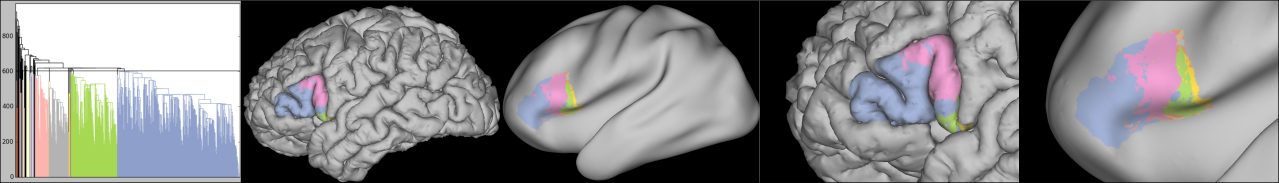
\includegraphics[width=\textwidth]{img/broca/logit_0.png}
    \caption{M\'etodo Logit sin preprocesamiento}
    \label{fig:dmri}
\end{minipage} ~
                                                                                                                        
\begin{minipage}[b]{\textwidth}
    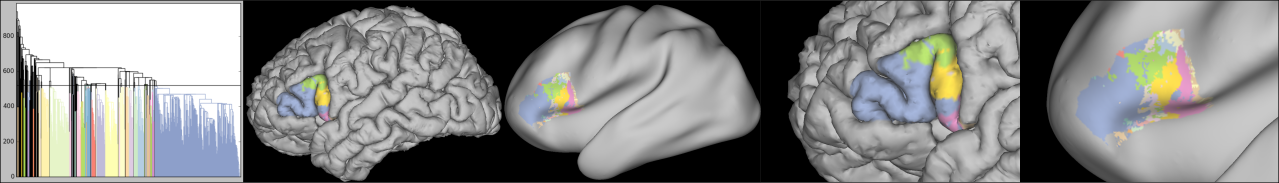
\includegraphics[width=\textwidth]{img/broca/logit_0_deep.png}
    \caption{M\'etodo Logit sin preprocesamiento, mayor profundidad en el 
            dendrograma}

\end{minipage} ~

\begin{minipage}[b]{\textwidth}
    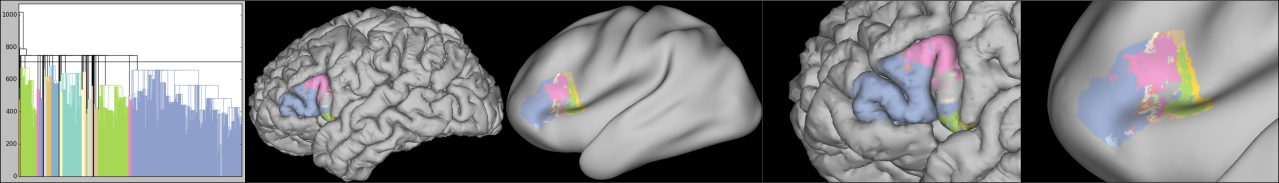
\includegraphics[width=\textwidth]{img/broca/logit_400.png}
    \caption{M\'etodo Logit, cuatrocientos pasos de preprocesamiento}

\end{minipage} ~

\begin{minipage}[b]{\textwidth}
    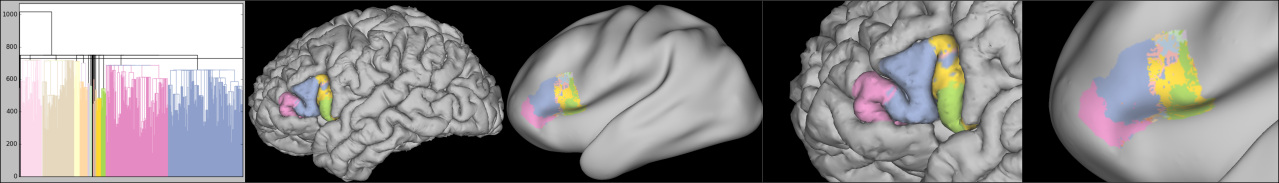
\includegraphics[width=\textwidth]{img/broca/logit_750.png}
    \caption{M\'etodo Logit, setecientos pasos de preprocesamiento}

\end{minipage} ~

\end{figure}


\subsection{Lado a lado}


\begin{figure}[h]

\begin{minipage}[h]{\textwidth}
    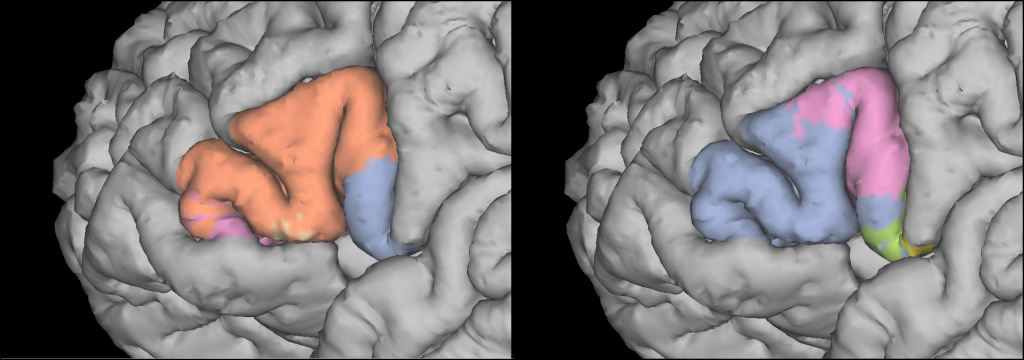
\includegraphics[width=\textwidth]{img/broca/vs_0.png}
    \caption{M\'etodo Moreno (izquierda) y Logit (derecha) sin preprocesamiento}
\end{minipage} ~

\end{figure}

\begin{figure}[h]                  

\begin{minipage}[h]{\textwidth}
    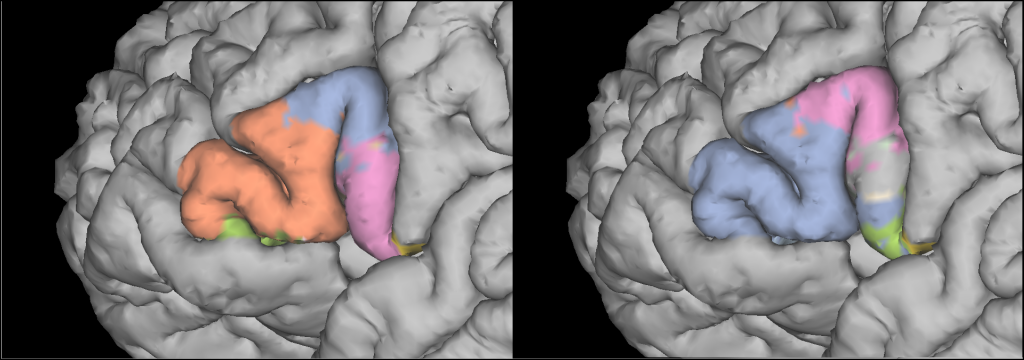
\includegraphics[width=\textwidth]{img/broca/vs_400.png}
    \caption{M\'etodo Moreno (izquierda) y Logit (derecha). Cuatrocientos pasos de preprocesamiento}
\end{minipage} ~

\end{figure}

\begin{figure}[h]

\begin{minipage}[h]{\textwidth}
    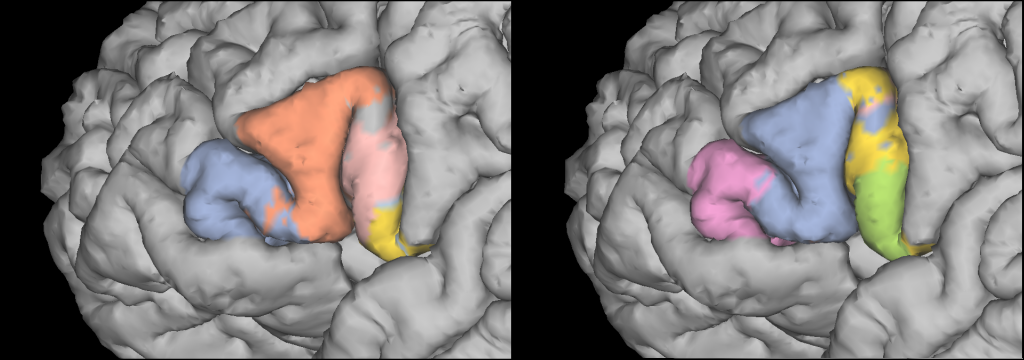
\includegraphics[width=\textwidth]{img/broca/vs_700.png}
    \caption{M\'etodo Moreno (izquierda) y Logit (derecha). Setecientos pasos de preprocesamiento}

\end{minipage} ~

\end{figure}
 


\section{Parcelando la corteza}

\subsection{Utilizando LogOdds}

\begin{figure}[h!]
                                                                                                                        
\begin{minipage}[b]{\textwidth}
    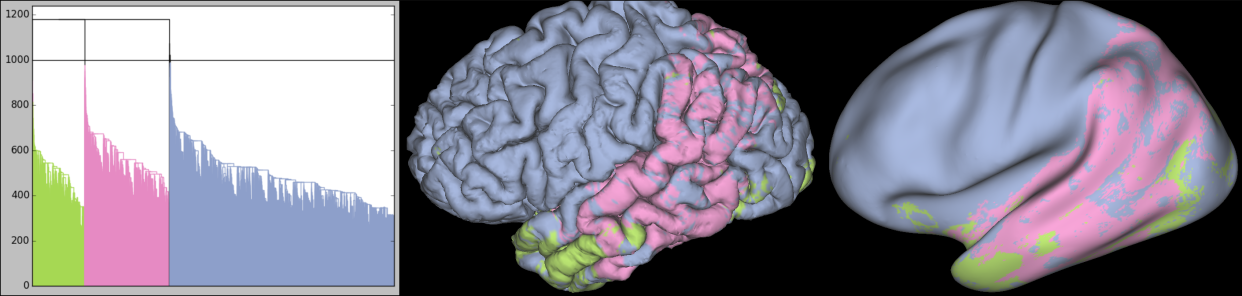
\includegraphics[width=\textwidth]{img/all_brain/logit_0.png}
    \caption{M\'etodo Logit sin preprocesamiento}
    \label{fig:dmri}
\end{minipage} ~
                                                                                                                        
\begin{minipage}[b]{\textwidth}
    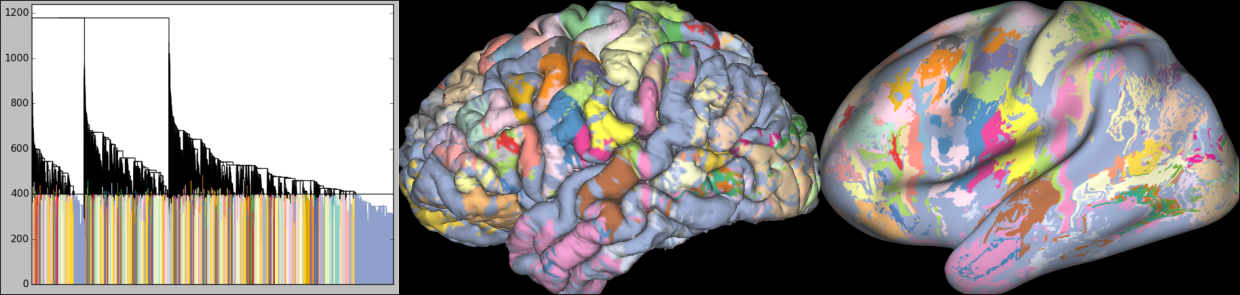
\includegraphics[width=\textwidth]{img/all_brain/logit_0_deep.png}
    \caption{M\'etodo Logit sin preprocesamiento, mayor profundidad en el 
            dendrograma}

\end{minipage} ~

\begin{minipage}[b]{\textwidth}
    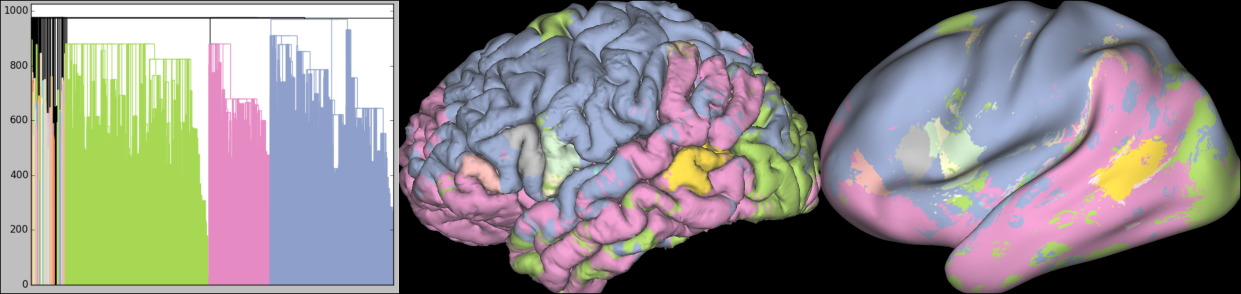
\includegraphics[width=\textwidth]{img/all_brain/logit_20000.png}
    \caption{M\'etodo Logit, veinte mil pasos de preprocesamiento}

\end{minipage} ~

\begin{minipage}[b]{\textwidth}
    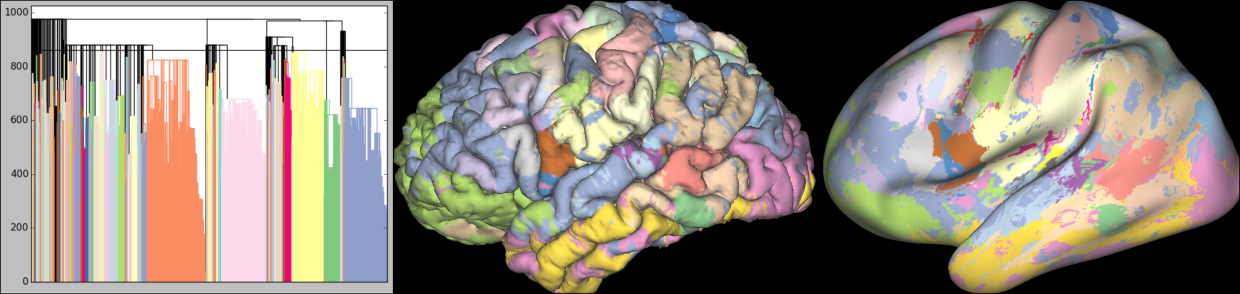
\includegraphics[width=\textwidth]{img/all_brain/logit_20000_deep0.png}
    \caption{M\'etodo Logit, veinte mil pasos de preprocesamiento, mayor 
             profundidad}
\end{minipage} ~

\begin{minipage}[b]{\textwidth}
    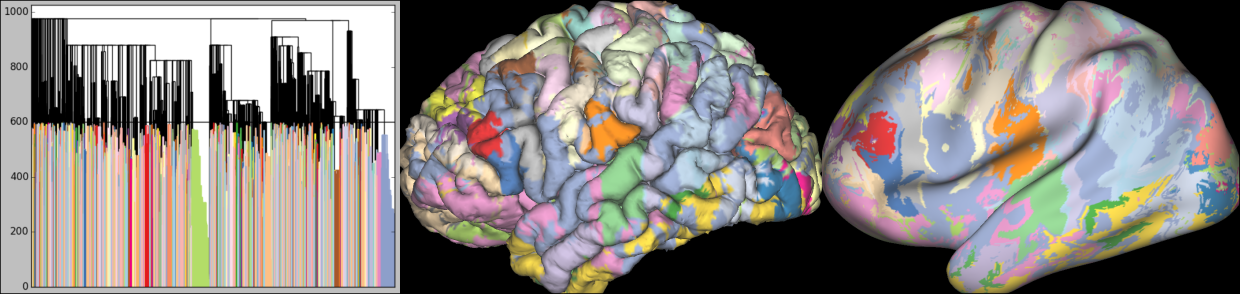
\includegraphics[width=\textwidth]{img/all_brain/logit_20000_deep1.png}
    \caption{M\'etodo Logit, veinte mil pasos de preprocesamiento, mayor 
             profundidad}
\end{minipage} ~


\end{figure}


\section{Correlato con otras parcelaciones de la literatura}
\label{sec:res_correlato}

Nuestro m\'etodo divide la corteza cerebral bas\'andose en un criterio
puramente estructural. En la literatura actual existen parcelaciones
basadas en otros criterios. A continuaci\'on contrastaremos nuestros 
resultados contra un atlas anat\'omico basado en Desikan \cite{Desikan2006}
y un estudio funcional realizado sobre el sujeto por Bach \cite{Barch2013}.

\subsection{Correlaci\'on anat\'omica}
\label{sec:corr_anatomica}

En la secci\'on \ref{sec:corteza_nuestro} parcelamos el hemisferio 
izquierdo de un sujeto con nuestro m\'etodo. Vamos a comparar el resultado
obtenido con el atlas anat\'omico basado en Desikan et al. 
\cite{Desikan2006}. La figura \ref{fig:an2pa} muestra el resultado de
proyectar algunas regiones anat\'omicas sobre las obtenidas con nuestro
m\'etodo. La figura \ref{fig:an2pa2} muestra solo las regiones que estaban
contenidas en su mayor\'ia dentro de estas proyecciones. Luego calculamos
que porcentaje de las parcelaciones quedaba dentro de las proyecciones;
que porcentaje quedaba fuera y cuantas quedaban dentro de una sola 
proyecci\'on. El $90\%$ del \'area de las 9 proyecciones est\'a pintada y
solo un $5\%$ del \'area de nuestras parcelas queda fuera de las
proyecciones. Las parcelas de nuestro m\'etodo que se encuentran en una
sola proyecci\'on representan el $88\%$ del \'area pintada. Las parcelas
que est\'an en dos regiones representan el $12\%$ restante. \\

Repetimos el procedimiento con los resultados obtenidos utilizando el 
m\'etodo de Moreno-Dominguez. Proyectamos el atlas anat\'omico sobre la
parcelaci\'on mostrada en la figura \ref{fig:moreno_corteza2}.
En este caso el $75\%$ del \'area de las 9 proyecciones est\'a pintada y 
un $15\%$ del \'area de las parcelas quedan fuera de las proyecciones. \\

\begin{figure}[h!]
    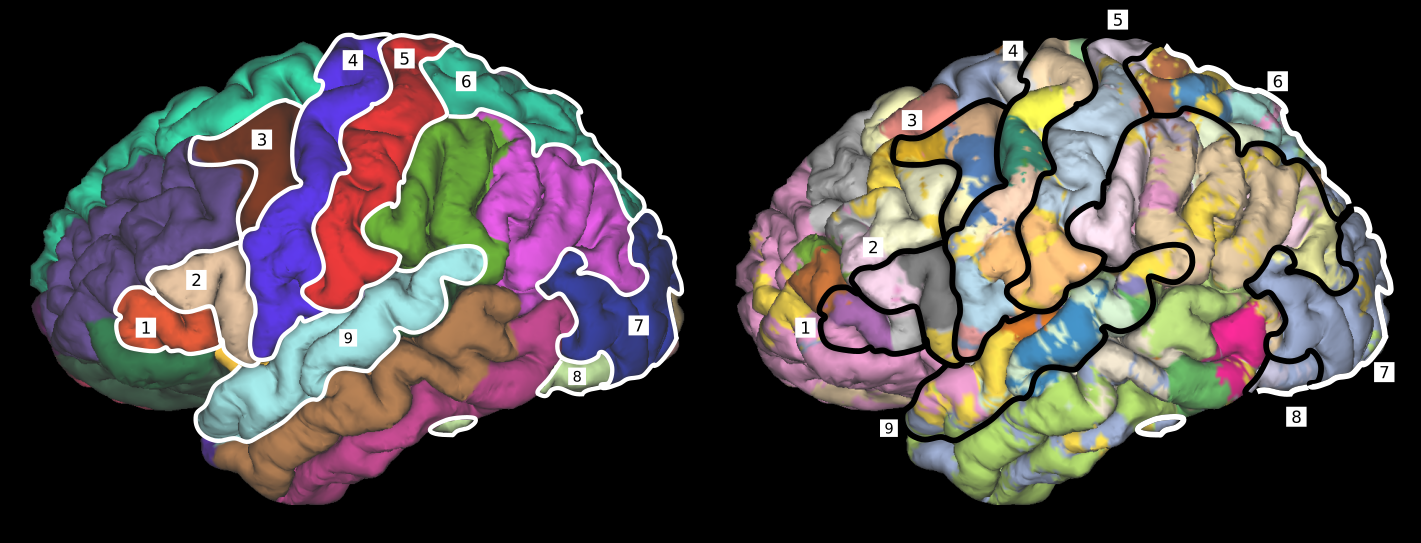
\includegraphics[width=\textwidth]{img/anatomica2parcelation.png}
    \caption{Proyecci\'on del atlas anat\'omico (izquierda) a la 
             parcelaci\'on obtenida (derecha). Regiones: 
             1. \textit{pars triangularis}; 2. \textit{pars opercularis};
             3. \textit{caudal middle frontal}; 
             4. \textit{precentral (\'area motora)}; 
             5. \textit{post central}; 6. \textit{superior parietal}; 
             7. \textit{lateral occipital}; 8. \textit{fusiform};
             9. \textit{superior temporal}.  }
    \label{fig:an2pa}
\end{figure}

\begin{figure}[h!]
    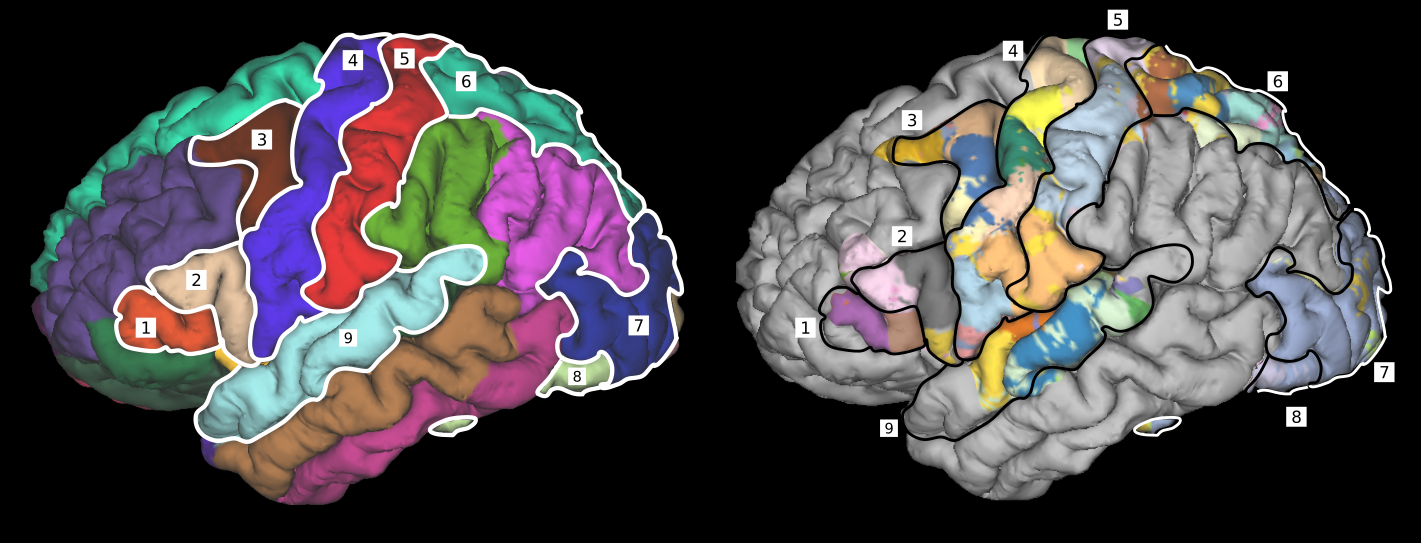
\includegraphics[width=\textwidth]{img/anatomica2parcelation2.png}
    \caption{Proyecci\'on del atlas anat\'omico (izquierda) a la 
             parcelaci\'on obtenida (derecha). Solo las parcelas contenidas
             en mayor proporci\'on fueron pintadas. Regiones: 
             1. \textit{pars triangularis}; 2. \textit{pars opercularis};
             3. \textit{caudal middle frontal}; 
             4. \textit{precentral (\'area motora)}; 
             5. \textit{post central}; 6. \textit{superior parietal}; 
             7. \textit{lateral occipital}; 8. \textit{fusiform};
             9. \textit{superior temporal}.  }
    \label{fig:an2pa2}
\end{figure}

\subsection{Correlaci\'on funcional}
\label{sec:corr_funcional}

Dentro del estudio funcional basado en Bach \cite{Barch2013} nos
enfocamos en las respuestas a los siguientes est\'imulos: mover la mano;
mover el pie; mover la lengua; reconocer formas y caras vistas con
anterioridad; clasificar un cuento breve dentro de dos categor\'ias y
resolver problemas aritm\'eticos simples. Por cada uno de estos est\'imulos
se cuenta con un mapa de \textit{z-scores}. Estos mapas representan la
correlaci\'on entre la activaci\'on de cada punto de la corteza con el 
est\'imulo. \\

\begin{figure}[h!]
    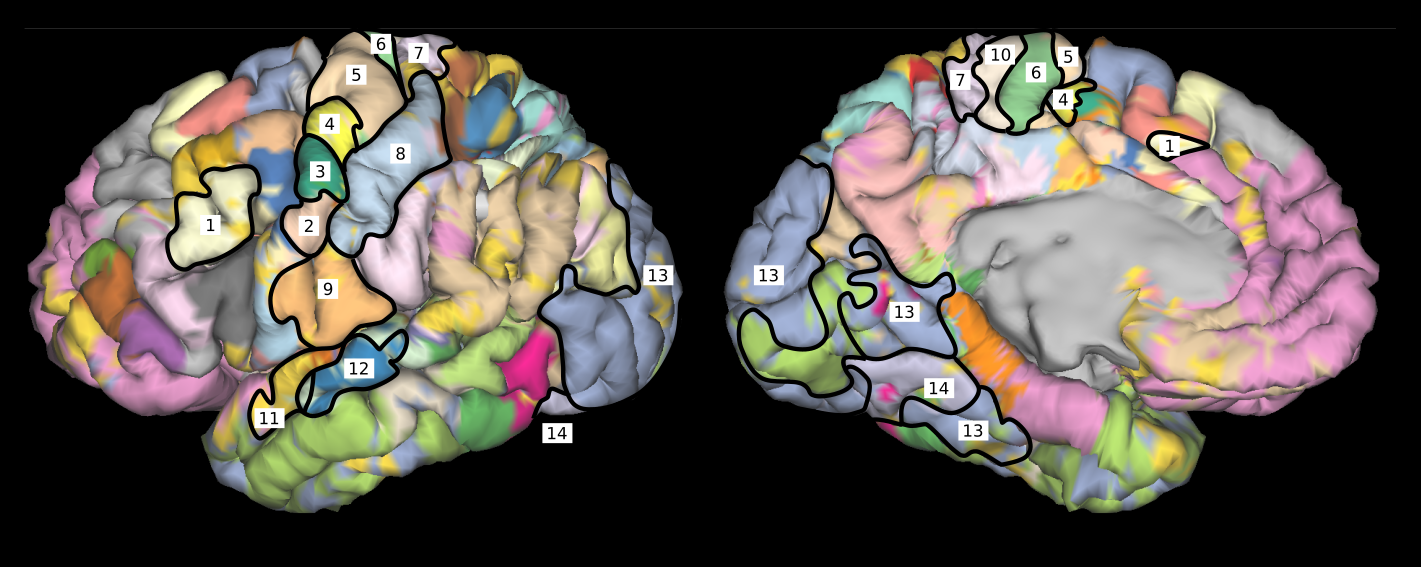
\includegraphics[width=\textwidth]{img/32k_labels.png}
    \caption{Parcelaci\'on obtenida utilizando nuestro m\'etodo. Se 
             etiquetaron algunas \'areas de inter\'es para comparar
             con un estudio funcional.}
    \label{fig:32k}
\end{figure}


\begin{figure}[h!]
    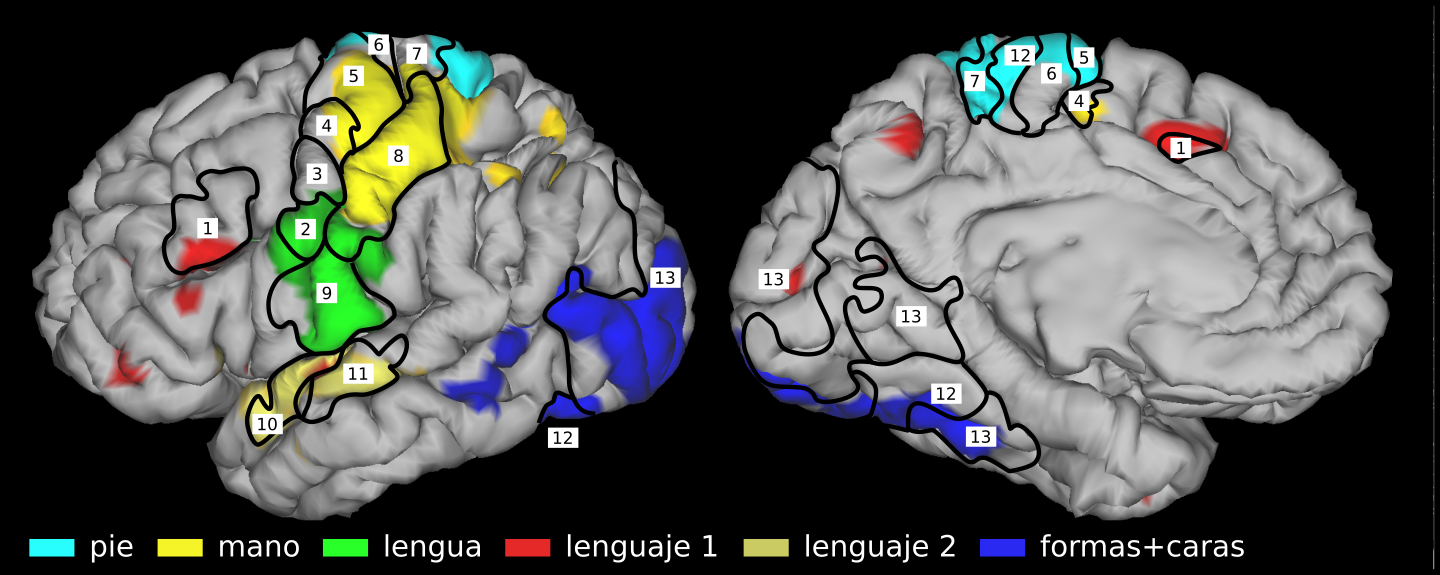
\includegraphics[width=\textwidth]{img/32k_z5.png}
    \caption{Proyecci\'on de 14 \'areas obtenidas con nuestro m\'etodo
             sobre los \textit{z-scores} mayores a $5$ de las activaciones
             funcionales.}
    \label{fig:32k_z5}
\end{figure}

\begin{figure}[h!]
    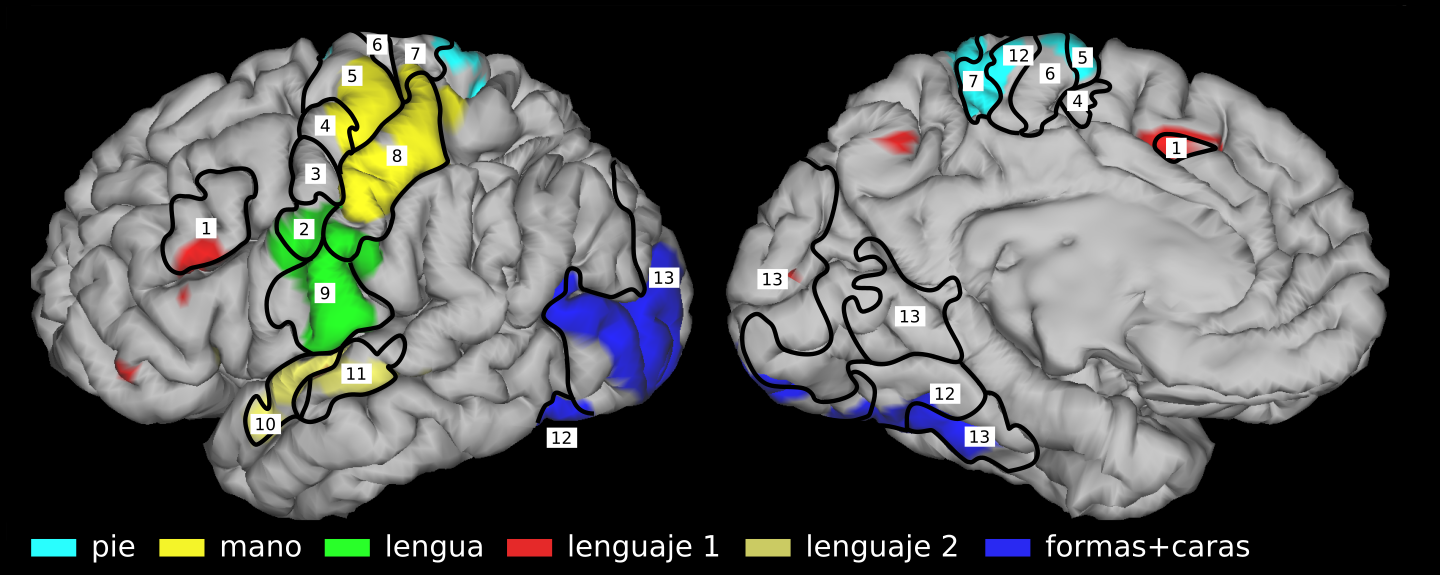
\includegraphics[width=\textwidth]{img/32k_z7.png}
    \caption{Proyecci\'on de 14 \'areas obtenidas con nuestro m\'etodo
             sobre los \textit{z-scores} mayores a $7$ de las activaciones
             funcionales.}
    \label{fig:32k_z7}
\end{figure}


Queremos comparar los mapas de \textit{z-scores} con una de las 
parcelaciones obtenidas mediante nuestro m\'etodo. Para ello primero
interpolamos la parcelaci\'on utilizada en la secci\'on anterior a la
superficie en que se encuentran los mapas. El resultado de dicha 
interpolaci\'on puede verse en la figura \ref{fig:32k}. Algunas regiones
de inter\'es fueron etiquetadas. La figura \ref{fig:32k_z5} muestra la
proyecci\'on de estas regiones sobre los \textit{z-scores} $ \geq 5$ de
los distintos mapas. La figura \ref{fig:32k_z7} muestra la proyecci\'on
sobre los \textit{z-scores} $ \geq 7$. \\

Utilizamos la ecuaci\'on \ref{eq:super} para estudiar la superposici\'on
entre nuestras regiones proyectadas y los \textit{z-scores}. La tabla 
\ref{tb:zscore5} muestra la superposici\'on entre las superficies de 
nuestra parcelaci\'on y los \textit{z-scores} $ \geq 5$.  La tabla 
\ref{tb:zscore7} muestra la superposici\'on entre las superficies de 
nuestra parcelaci\'on y los \textit{z-scores} $ \geq 7$. En cada columna
se resalt\'o el valor mas grande. Esto es, el valor de la parcela que
mayor superficie compart\'ia con cada mapa de activaci\'on.  \\
 
\begin{table}[]
\centering
\begin{tabular}{|l|l|l|l|l|l|l|}
\hline
   & pie   & mano  & lengua & matem\'atica & cuento & formas \\ \hline
1  & 0     & 0     & 0      & 0.276      & 0      & 0      \\ \hline
2  & 0     & 0     & 0.311  & 0          & 0      & 0      \\ \hline
3  & 0     & 0     & 0      & 0          & 0      & 0      \\ \hline
4  & 0     & 0.172 & 0      & 0          & 0      & 0      \\ \hline
5  & 0.177 & 0.321 & 0      & 0          & 0      & 0      \\ \hline
6  & 0.201 & 0     & 0      & 0          & 0      & 0      \\ \hline
7  & 0.231 & 0.044 & 0      & 0          & 0      & 0      \\ \hline
8  & 0     & {\bf 0.590} & 0.139  & 0          & 0      & 0      \\ \hline
9  & 0     & 0     & {\bf 0.610}   & 0          & 0      & 0      \\ \hline
10 & {\bf 0.330}  & 0     & 0      & 0          & 0      & 0      \\ \hline
11 & 0     & 0     & 0      & 0          & {\bf 0.606}  & 0      \\ \hline
12 & 0     & 0     & 0      & 0          & 0.454  & 0      \\ \hline
13 & 0     & 0     & 0      & 0          & 0      & {\bf 0.491}  \\ \hline
14 & 0     & 0     & 0      & 0          & 0      & 0.154  \\ \hline
\end{tabular}
\caption{Relaci\'on entre las \'areas de cada parcela y los mapas de
         activaci\'on con $zscore > 5$. Los valores m\'aximos de cada 
         columna fueron resaltados.}
\label{tb:zscore5}         
\end{table}


\begin{table}[]
\centering

\begin{tabular}{|l|l|l|l|l|l|l|}
\hline
   & pie   & mano  & lengua & matem\'atica & cuento & formas \\ \hline
1  & 0     & 0     & 0      & {\bf 0.419} & 0     & 0      \\ \hline
2  & 0     & 0     & 0.323  & 0          & 0      & 0      \\ \hline
3  & 0     & 0     & 0      & 0          & 0      & 0      \\ \hline
4  & 0     & 0.115 & 0      & 0          & 0      & 0      \\ \hline
5  & 0.141 & 0.341 & 0      & 0          & 0      & 0      \\ \hline
6  & 0.095 & 0     & 0      & 0          & 0      & 0      \\ \hline
7  & {\bf 0.377} & 0.040 & 0      & 0          & 0      & 0      \\ \hline
8  & 0     & {\bf 0.669} & 0.147  & 0          & 0      & 0      \\ \hline
9  & 0     & 0     & {\bf 0.629}  & 0          & 0      & 0      \\ \hline
10 & 0.240 & 0     & 0      & 0          & 0      & 0      \\ \hline
11 & 0     & 0     & 0      & 0          & {\bf 0.715}  & 0      \\ \hline
12 & 0     & 0     & 0      & 0          & 0.458  & 0      \\ \hline
13 & 0     & 0     & 0      & 0          & 0      & {\bf 0.428}  \\ \hline
14 & 0     & 0     & 0      & 0          & 0      & 0.154 \\ \hline
\end{tabular}
\caption{Relaci\'on entre las \'areas de cada parcela y los mapas de
         activaci\'on con $zscore > 7$. Los valores m\'aximos de cada 
         columna fueron resaltados.}
\label{tb:zscore7}         
\end{table}


